% !TeX program = xelatex

\documentclass[12pt,a4paper]{article}

\usepackage[UTF8,scheme=chinese]{ctex}
\usepackage{xeCJK}
\usepackage{url}
\usepackage{hyperref}
\usepackage{graphicx}
\usepackage{geometry}
\usepackage{setspace}
\usepackage{amsmath}
\usepackage{amsfonts}
\usepackage{amssymb}
\usepackage{cite}
\usepackage{fontspec}

\setmainfont{Times New Roman}

\setCJKmainfont{標楷體}

\newCJKfontfamily\kaiFakeBold[FakeBold=2]{標楷體}

\makeatletter
\renewcommand\bfseries{
  \kaiFakeBold
  \fontseries\bfdefault\selectfont
}
\makeatother

\ctexset{
    contentsname={目錄},
    listfigurename={圖目錄},
    listtablename={表目錄},
    figurename={圖},
    tablename={表},
    abstractname={摘要},
    indexname={索引},
    appendixname={附錄},
    bibname={參考文獻}
}

% 基本套件


% 頁面設定
\geometry{
    left=3cm,
    right=2cm,
    top=2.5cm,
    bottom=2.5cm
}

% 行距設定
\onehalfspacing

\begin{document}
\begin{titlepage}

	\centering
	\vspace*{2cm}
	
	{\Large 國立臺灣海洋大學\\[0.5cm]資訊工程系專題報告 \par}
	
	\vspace*{1cm}
	{\Huge 智慧化船舶群集搜救模擬系統 \par}
	
	\vfill
	
	{\Large 指導教授:鄭錫齊 教授 \par}
	\vspace*{1cm}
	\begin{tabular}{lll}
	學號 & 姓名 & E-mail \\
	\hline
	\end{tabular}

	\vspace*{1cm}
	{\Large 中華民國\ 114 年\ 9 月\ 21 日 \par}

\end{titlepage}

% 摘要
\vspace*{0.3\textheight}
\begin{abstract}
海上搜救任務面臨著範圍廣闊、海象險惡、時間緊迫等嚴峻挑戰。為應對此一難題,本專案建構了一套「智慧化船舶群集搜救模擬系統」。系統核心旨在模擬並最佳化真實的搜救作業流程:首先,依據目標可能區域進行高效的網格化分割;接著,指揮調度多艘船隻構成的搜救群集,對各區塊展開平行搜索,以最大化覆蓋率並縮短搜尋時間。我們在 Unity 與 Crest 物理引擎打造的擬真海洋環境中,採用 SAC 深度強化學習演算法,賦予每艘搜救船隻在複雜風浪中自主執行精密搜索路徑、並規避動態障礙物的能力。本專案旨在評估此 AI 驅動的搜救群集,在不同搜救情境下,對於提升目標發現成功率、縮短搜救時間的實際成效,為未來智慧化海上應急響應系統提供關鍵的模擬驗證。
\end{abstract}

\centerline{\textbf{關鍵詞:} 船舶群集、搜救系統、深度強化學習、多智慧體系統、海洋模擬}

\newpage

% 目錄
\tableofcontents
\newpage

% 正文開始
\section{緒論}

\subsection{研究背景與動機}
海洋覆蓋地球表面超過七成,是全球貿易、資源開發與休閒活動的核心場域。然而,隨著海上交通與作業日益頻繁,船舶事故、惡劣氣候與人員落水的風險持續上升。一旦發生事故,搜救(Search and Rescue, SAR)行動成為攸關人命的即時挑戰,其中「救援時間」決定了受困者的生存率。

傳統搜救模式仰賴人員經驗與指揮調度,在大範圍海域與高風險環境下常受限於人力與效率。隨著人工智慧(AI)、自主系統(Autonomous Systems)與高擬真模擬技術的成熟,發展基於智慧化與自主化的搜救系統已成為突破現有困境的契機。自主船舶群集可藉由耐航性、即時協作與精確導航,提升搜救任務的速度與覆蓋範圍,進而增加受困人員的獲救機率。本研究即在此背景下展開。

\subsection{問題陳述}
雖然自主船舶與強化學習的應用展現巨大潛力,但在搜救場景中仍面臨多重挑戰:

\begin{enumerate}
\item \textbf{搜索效率不足}:傳統搜索在大範圍海域下難以兼顧效率與覆蓋率。
\item \textbf{環境動態與不確定性}:風浪與洋流使船隻航行與感測受干擾,增加搜尋難度。
\item \textbf{群集協同複雜性}:多艘船隻需避免重複搜索、確保安全並即時共享資訊。
\item \textbf{時間壓力與決策挑戰}:有限時間內需快速分配資源並做出最佳判斷,錯誤可能導致錯失救援時機。
\end{enumerate}

因此,有必要建構一個智慧化模擬系統,以驗證不同策略並最佳化搜救行動。

\subsection{研究目的}
本研究的主要目標在於建立一個「智慧化船舶群集搜救模擬系統」,具體目的如下:

\begin{itemize}
\item \textbf{建立高擬真虛擬環境}:以 Unity 與 Crest 套件模擬真實海象與物理效果,作為測試平台。
\item \textbf{開發自主搜救智慧體}:利用深度強化學習演算法,訓練船舶於動態環境中進行自主導航與避障。
\item \textbf{設計群集協同策略}:透過分區搜尋與任務分配,提升多船協同效率,避免重複與衝突。
\item \textbf{效能評估與驗證}:以模擬實驗檢驗系統在搜尋成功率、平均搜救時間與協同效率上的成效。
\end{itemize}

\subsection{專題架構}
本專題共分為七章,內容安排如下:

\begin{itemize}
\item \textbf{第一章 緒論}:說明研究背景、問題陳述、研究目的與章節安排。
\item \textbf{第二章 文獻回顧與討論}:探討海上搜救、強化學習、多代理人系統與模擬相關研究。
\item \textbf{第三章 相關使用技術介紹}:介紹研究所採用之深度強化學習演算法(SAC)、Unity3D、ML-Agents 與 Crest 模擬套件。
\item \textbf{第四章 系統設計與技術實作}:說明系統硬體與軟體環境、系統架構設計、強化學習架構與套件整合方法。
\item \textbf{第五章 實驗設計與結果分析}:呈現實驗設計、數據收集與結果分析,驗證系統效能。
\item \textbf{第六章 結論與未來發展}:總結研究成果,並提出研究限制與未來可能發展。
\item \textbf{第七章 參考資料}:列出研究所參考之文獻與資料來源。
\end{itemize}

\newpage

\section{文獻回顧與討論}

\subsection{海上搜救相關研究}

\subsubsection{傳統海上搜救方法}
傳統的海上搜救方法在《IAMSAR 操作手冊》\cite{IAMSAR2008} 中有明確規範,常見的類型有:
\begin{itemize}
	\item \textbf{Expanding square search(擴展方形搜尋)}
	\begin{itemize}
		\item 適用於目標位置大致已知、中等範圍的搜尋。
		\item 搜尋點從基準點開始搜尋,每次往前一段距離後轉向 90 度,每次轉向航段都會逐漸加長。
		\item 需要準確的導航系統。
	\end{itemize}
	\item \textbf{Sector search(扇形搜尋)}
	\begin{itemize}
		\item 適用於目標位置明確、小範圍的搜尋。
		\item 搜尋方式由基準點為圓心,進行放射狀的搜尋。
		\item 最多只能由一艘船與一架飛機分別進行搜尋。
	\end{itemize}
	\item \textbf{Parallel sweep search(平行航線搜尋)}
	\begin{itemize}
		\item 適用於目標位置未知、大範圍的搜尋。
		\item 搜尋區域被劃分為多個子區域,由不同的船舶分工搜尋,每個子區域的搜尋航線互相平行,並與海流方向一致。
		\item 由於派出的單位較多,因此需要消耗大量的資源。
	\end{itemize}
\end{itemize}

\begin{figure}[h]
    \centering
    \begin{minipage}[t]{0.3\textwidth}
        \centering
        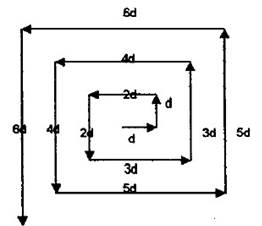
\includegraphics[width=\textwidth]{image/ExpandingSquareSearch.png}
        \caption{擴展方形搜尋}
    \end{minipage}%
    \hfill
    \begin{minipage}[t]{0.3\textwidth}
        \centering
        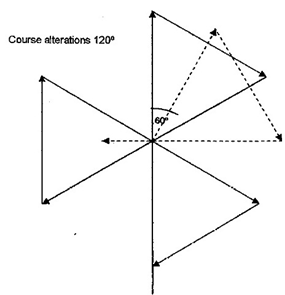
\includegraphics[width=\textwidth]{image/SectorSearch.png}
        \caption{扇形搜尋}
    \end{minipage}%
    \hfill
    \begin{minipage}[t]{0.3\textwidth}
        \centering
        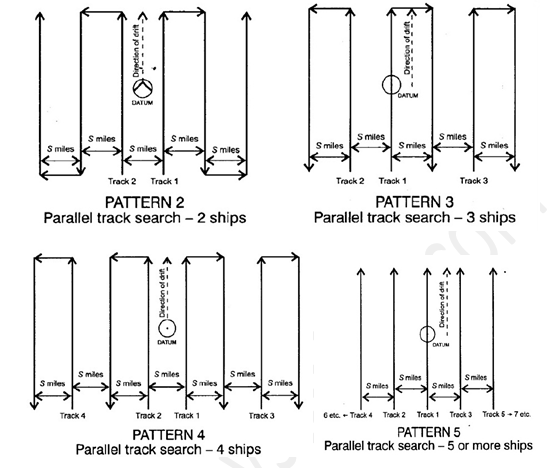
\includegraphics[width=\textwidth]{image/ParallelSweeepTrack.png}
        \caption{平行航線搜尋}
    \end{minipage}
\end{figure}


\subsubsection{傳統方法的限制與挑戰}
\begin{itemize}
  \item \textbf{安全風險}:傳統的搜救方式需要出動大量的人員與船舶,如在極端天候可能會造成額外的風險。
  \item \textbf{人力與資源消耗}:以平行航線為例,雖然能夠覆蓋較大的範圍,但同時也需要使用大量的船舶及人員,而搜救成本也隨之增加。
  \item \textbf{搜尋效率受限}:擴展正方形、扇形搜尋雖然成本相較為低廉,然而其搜尋範圍相對有限,並且在海流及海風的影響下,航線容易偏移,降低搜尋效率。
  \item \textbf{時效性不足}:當目標位置未知且搜尋範圍過大,傳統的人工搜尋方法往往很難在黃金救援期間完成全面搜尋。
\end{itemize}

\subsubsection{技術發展}
隨著科技進步,傳統搜救方式的限制逐漸被新技術所補足:
\begin{itemize}
  \item \textbf{無人機}:具備高機動性,能在短時間內對大範圍的海域進行空中偵查。
  \item \textbf{自主船舶}:可執行長時間、低成本的搜尋,降低人員風險與油料消耗。使用群集作業可以補足平行航線搜尋的缺點,在維持大範圍的情況下同時減少搜尋成本。
  \item \textbf{混和搜救系統}:結合有人、無人船舶及無人機,形成「立體化」的搜尋網路。有人單位可以集中精力於高價值決策或特殊任務,無人單位負責長時間及大範圍的搜尋。
\end{itemize}

\subsection{自主船舶系統現代應用}
隨著無人化技術的推進,USV 在海洋產業中逐漸成熟並投入實際應用。主要集中在以下的面向:
\begin{itemize}
  \item \textbf{任務自動化與導航精準度}:透過高精度 GPS 與自主導航演算法,使船舶能在無人操控下完成大範圍的搜尋與調查。
  \item \textbf{能源與續航力優化}:積極推動電力及太陽能的使用,用以滿足長時間海上作業的需求。
  \item \textbf{安全與可靠性}:增設船體健康監控、故障預警與各種感測器,以即時偵測船體外部環境進行自主避障。
  \item \textbf{應用多元化}:涵蓋貨運、離岸風電運維、海洋調查與急難救助等。
\end{itemize}

\paragraph{相關應用案例}
\begin{itemize}
  \item Yara Birkeland:全球首艘全電動無人貨櫃船,展現大型自主船舶的商轉潛力。
  \item 日本 MEGURI 2040 計畫:推動多艘無人渡輪與貨船運行,測試長距離自主航行能力。
  \item 英國 Rolls-Royce、韓國現代重工:積極投入智慧船舶與自主航行技術。
\end{itemize}

\subsection{深度強化學習於自主導航領域之研究}

\subsubsection{傳統演算法與限制}
在自主導航(Autonomous Navigation)領域中,傳統的路徑規劃方法如 A*、Dijkstra 與快速隨機樹(Rapidly-exploring Random Tree, RRT),一直是最為基礎且廣泛使用的演算法。

\begin{itemize}
  \item \textbf{Dijkstra}:以圖論為基礎,透過計算從起點到所有節點的最短距離來確保最短路徑的正確性。此方法在靜態地圖或事先已知環境中具備嚴謹性,但計算複雜度高,且在動態情境下缺乏快速更新能力,難以應對環境中即時出現的障礙物或突發狀況。
  \item \textbf{A*}:結合啟發式函數與 Dijkstra 的最短路徑搜尋概念,能在靜態環境下有效找到近似最優路徑。其優點在於搜尋效率高,且能保證找到全域最優解。然而在動態環境中,當障礙物或目標位置發生變化時,A* 必須重新進行全域規劃,導致即時性不足。
  \item \textbf{RRT}:屬於取樣式(sampling-based)的規劃方法,能在高維空間中迅速探索可行路徑,特別適合處理複雜的路線規劃。然而其生成的路徑往往並非最優,且需要額外優化程序。同時,RRT 在面對動態障礙物時也需頻繁重新生成樹狀結構,導致計算負擔增加。
\end{itemize}

\noindent 綜觀而言,傳統演算法的主要限制包括:
\begin{itemize}
  \item 缺乏即時適應性:當環境發生變化(如動態障礙物、移動目標)時,需重新規劃路徑,反應速度不足。
  \item 計算負擔大:在高維、複雜或大規模環境下,演算法的計算時間與記憶體需求急遽增加。
  \item 難以處理不確定性:傳統規劃多依賴完整或靜態的環境資訊,在感測器噪音、動態行人或其他不確定因素下,效能顯著下降。
\end{itemize}

因此,雖然傳統方法在靜態場景中表現穩健,但在動態且不確定的自主導航環境中,往往無法滿足即時決策與適應性需求,這正是深度強化學習(Deep Reinforcement Learning, DRL)開始受到重視的原因。


\subsubsection{深度強化學習的突破}
為克服傳統演算法在動態環境下的不足,深度強化學習(Deep Reinforcement Learning, DRL)成為自主導航研究中的重要突破。與 A*、Dijkstra、RRT 等需要完整環境模型並重新規劃的方式不同,DRL 採用 trial-and-error(嘗試錯誤)學習機制,透過與環境的交互不斷更新策略(policy),進而實現動態決策與即時反應。

\paragraph{(1) 自主學習與即時決策}
DRL 將強化學習(Reinforcement Learning, RL)的價值函數或策略函數,結合深度神經網路的表徵能力,使智能體能在高維感知輸入(如 LiDAR、相機影像)下直接學習導航策略。這種方式無需依賴精確的地圖建模或完整環境資訊,而是透過即時觀測與回饋,逐步形成能適應不同情境的決策能力。

\paragraph{(2) 處理動態與不確定性}
相較於傳統演算法須頻繁重新規劃路徑,DRL 在訓練過程中即已接觸到各種動態障礙物與隨機擾動,因而具備在未知或變化環境中快速調整的能力。例如,當遇到突然出現的障礙物時,智能體能即時採取繞行或減速等動作,而不必從頭運算整條路徑。

\paragraph{(3) 泛化與適應性}
透過大量訓練資料與模擬環境,DRL 模型能學會在不同場景間泛化。例如,同一策略可在室內走廊、室外道路或不同地圖配置中應用,具備比傳統演算法更強的靈活性。這使得 DRL 特別適合應用於具有高度不確定性的場景,如自駕車或自主移動機器人。

\noindent 綜合而言,DRL 透過嘗試錯誤式的學習框架,彌補了傳統演算法在動態性、即時性與不確定性上的不足,為自主導航帶來全新的解決方案。這些優勢使其在自駕車、無人機以及服務型機器人等領域展現出廣泛的應用潛力。

\subsubsection{核心演算法應用}
\begin{itemize}
  \item \textbf{DQN(Deep Q-Network)}:為傳統 Q-Learning 的延伸,利用深度神經網路來近似 Q-Value,解決傳統 Q-Table 無法應付大型或連續狀態空間的問題。
  \item \textbf{PPO(Proximal Policy Optimization)}:一種在策略空間進行優化的演算法,核心概念是在保證新的策略與舊的策略差異不會太大的前提下,尋找一個性能更好的策略。
  \item \textbf{SAC(Soft Actor-Critic)}:基於 Actor-Critic 的演算法,融合最大熵強化學習,在學習高回報策略的同時,鼓勵策略保持隨機性以提升探索能力,適合高維度與連續動作空間。
\end{itemize}

\newpage

\paragraph{案例分析}
\begin{itemize}
  \item 無人車模擬環境中的 DQN 應用:一項研究探討了 DQN 在無人車模擬環境中的應用,特別是在安全、正常與激進駕駛模式下的表現。結果顯示,DQN 能夠有效學習並適應不同駕駛模式。\cite{rybchak2024}
  \item 無人機應急導航:斯坦福大學的研究團隊開發了一個基於 DQN 和 SAC 的無人機導航系統,用於應急情境中的快速部署與導航。\cite{greenberg}
\end{itemize}

\subsection{模擬平台與方法比較}

\begin{itemize}
  \item \textbf{模擬平台比較}:
  為了模擬現實自主船舶在大範圍海域的搜救能力,本專案需一個能夠模擬大範圍海域、高擬真波浪、同時支援運行自主航行演算法的測試平台。主要平台比較如下:
  \begin{itemize}
    \item \textbf{Unity}:跨平台、視覺效果強、支援 Crest 波浪插件。限制在物理模擬精度相較專業模擬器稍差。適用於大規模海洋場景、波浪及執行群集航行策略演算法。
    \item \textbf{Gazebo}:與 ROS 深度整合、演算法測試方便。限制在大規模海洋場景支援有限,難以呈現複雜海況。
    \item \textbf{MORSE (Modular OpenRobots Simulation Engine)}:研究導向,支援機器人學術模擬與感測器模擬。限制為社群小、更新頻率低、擴充性較差,僅適合學術性演算法測試。
    \item \textbf{Webots}:教育與研究常用,內建機器人模型與控制介面。限制在大範圍海洋模擬上表現不足,適合小型場景。
  \end{itemize}
  
  \item \textbf{Unity 與 Crest 的優勢}:
  \begin{itemize}
    \item \textbf{真實感佳}:Crest 基於 FFT 波譜法生成海浪,模擬效果逼真。
    \item \textbf{即時渲染}:支援 GPU 加速,可進行大規模的波浪實時模擬。
    \item \textbf{無縫整合}:Crest 作為 Unity 插件,不需要額外轉換資料或外部軟體支援。
  \end{itemize}
  綜合比較:Unity + Crest 能夠同時滿足海洋擬真、模擬規模及自主船舶的控制測試需求,因此我們選擇其作為首選模擬環境。
\end{itemize}

\subsection{代理人系統}

\begin{itemize}
  \item \textbf{單代理人系統(Single-Agent Systems, SAS)}:
  單代理人系統是指整個任務由一個代理人獨立完成。適用於任務範圍小、環境單純的情境,成本較低廉,但在大範圍及複雜環境下效率受限。
  
  \item \textbf{多代理人系統(Multi-Agent Systems, MAS)}:
  MAS 由多個自主代理人組成,每個代理人能獨立運作,並透過協作、競爭等方式完成各自或共同的任務目標。常應用於大規模、分散且動態的環境。其訓練難度較高,主要挑戰包括:
  \begin{itemize}
    \item \textbf{動態環境}:每個代理人在學習中會改變策略,導致環境不斷變化,不可預測且難以捉摸。
    \item \textbf{部分觀測與不確定性}:每個代理人只能感知局部環境資訊,需要推斷其他代理人的狀態及意圖。
    \item \textbf{協作與衝突}:代理人需要學習如何協作及分工,避免互相干擾。
  \end{itemize}
\end{itemize}

\subsection{文獻總結與研究方向}

\begin{itemize}
  \item \textbf{研究缺口}:缺乏針對「智慧化船舶群集」在海洋環境下進行搜救的模擬平台。
  \item \textbf{本研究貢獻}:
  \begin{itemize}
    \item 建立結合 Unity 與 Crest 的海洋高擬真測試平台。
    \item 開發基於 SAC 的自主船舶智慧體。
    \item 提出可行的群集搜尋策略,並透過模擬驗證效能。
  \end{itemize}
\end{itemize}

\section{相關使用技術介紹}
\subsection{深度強化學習核心演算法 — Soft Actor-Critic (SAC)}
Soft Actor-Critic (SAC) 是一種基於最大熵強化學習(maximum entropy RL)的演算法,其核心思想是在策略學習過程中同時最大化期望回報與策略熵。換言之,SAC 不僅追求高獎勵,也鼓勵策略在決策時保持隨機性,以提升探索能力與穩定性。透過在目標函數中引入熵正則項,SAC 能在「利用高獎勵行為」與「保留行為多樣性」之間取得平衡,最終使得代理人在不確定或動態環境中能學習到更穩定且具泛化性的策略。
\\ \par
SAC 建立在 actor-critic 架構 上:
\begin{enumerate}
	\item \textbf{Actor(策略網路)}:輸出參數化的隨機策略,通常以高斯分布建模,並透過重參數化技巧進行動作取樣,使策略更新可微分。
	\item \textbf{Critic(價值網路)}:使用兩個 Q 函數(twin Q-networks)以降低過度估計偏差,透過軟化的貝爾曼方程(soft Bellman backup)學習回報與熵加權後的價值。
	\item \textbf{熵正則項}:在目標函數中加入策略熵,使代理人不僅追求獎勵最大化,也保持行為的隨機性,以鼓勵探索並避免過早收斂。
	\item \textbf{自動調整溫度參數}:SAC 可動態調整溫度係數 α,自適應地平衡「利用」與「探索」,避免需要手動調參。
\end{enumerate}

SAC 演算法有以下優點:
\begin{itemize}
	\item \textbf{穩定的訓練過程}:SAC 採用經驗回放,在每次更新時只隨機抽取一小部分過往經驗來訓練,而不是僅依賴即時資料。這樣能打破資料間的相關性,降低方差,使訓練過程更平滑與穩定。
	\item \textbf{避免過度收斂,提升探索性}:SAC 在目標函數中引入「熵」正則項,鼓勵策略在學習過程中保持隨機性,避免過早收斂到次佳解。
	\item \textbf{偏差控制與高效學習}:使用 double Q-networks 減少了價值高估問題。
	\item \textbf{自動化探索 - 利用平衡}:SAC 允許自動調整溫度參數 α,動態平衡「追求回報」與「保持隨機性」,減少對超參數的敏感度。
\end{itemize}

\subsection{Unity3D 開發引擎}

Unity3D(以下簡稱 Unity)是一款跨平台的即時 3D 開發引擎,廣泛應用於遊戲開發、虛擬實境(VR)、擴增實境(AR)、模擬器以及互動式應用。

Unity 的核心特點包括:

\begin{itemize}
    \item \textbf{跨平台支援}:開發者可以一次編寫程式碼,將應用部署到 Windows、MacOS、iOS、Android、WebGL、PlayStation、Xbox 等多種平台。
    \item \textbf{可視化編輯器}:提供直觀的場景設計與資源管理介面,方便開發者進行場景佈置、動畫製作與物理模擬。
    \item \textbf{C\# 腳本語言}:使用 C\# 編寫遊戲邏輯與互動行為,並支持與外部系統進行資料交換。
    \item \textbf{豐富的資源與插件}:Unity 提供官方資源商店,開發者可快速取得模型、材質、插件及範例專案,加速開發流程。
\end{itemize}

由於 Unity 支援物理模擬、碰撞檢測、光影渲染以及高自由度場景控制,因此除了遊戲開發,Unity 也被廣泛應用於機器人模擬、數位孿生、教育訓練與科研領域。



\subsection{ML-Agents}
ML-Agents(Unity Machine Learning Agents Toolkit)是 Unity 官方推出的開源工具套件,主要用於將 Unity 環境轉化為可供智能體訓練的模擬環境。其主要功能是讓開發者在 Unity 中建立智能體(Agent)並進行機器學習或強化學習的訓練。
\\ \par
ML-Agents 的核心特點包括:

\begin{itemize}
	\item \textbf{智能體與環境建模}:在 Unity 場景中建立智能體,定義其觀察、可執行動作以及獎勵函數。
	
	\item \textbf{Python 訓練介面}:提供 Python API 與 PyTorch 支援,可使用多種強化學習算法進行訓練,並與 Unity 環境實時交換資料。
	
	\item \textbf{支援多種學習模式}:
	
	\begin{itemize}
	\item 強化學習(Reinforcement Learning, RL):透過試錯學習優化策略。
	
	\item 模仿學習(Imitation Learning):透過人類示範數據訓練智能體模仿行為。
	
	\item 自我對弈(Self-Play):適用於對抗型任務,智能體透過與自己或其他智能體對弈學習策略。
	\end{itemize}	

	\item \textbf{模型匯出與部署}:訓練完成的策略可以匯出為模型(如 ONNX 格式),直接在 Unity 環境中執行,無需依賴 Python 訓練器。
\end{itemize}

ML-Agents 套件的引入,使 Unity 不僅可以用於互動式模擬,也可作為智能體學習與研究的高效平台,特別適合機器人控制、自駕模擬以及複雜行為策略的研究。


\subsection{Crest 海洋環境模擬套件}
Crest 是一款專為 Unity3D 開發的高品質海洋渲染與模擬插件,用於生成逼真的水面效果和動態海洋環境。它廣泛應用於遊戲開發、虛擬現實、模擬器以及互動式應用中,能夠提供高度真實的水面視覺效果和物理互動。

\subsubsection{核心特點}
\begin{itemize}
    \item \textbf{逼真波浪模擬}:使用 FFT(Fast Fourier Transform)生成自然海浪,可模擬遠景大波和近景小波紋。
    \item \textbf{水面光影效果}:支援動態反射、折射及水下光照,呈現真實光影交互。
    \item \textbf{物理互動}:支援物體與水面的動態交互,如浮動物體、波紋生成和水面擾動。
    \item \textbf{性能優化}:提供 LOD(Level of Detail)管理與 GPU 加速技術,在大規模水域場景下保持高效能。
    \item \textbf{可擴展性}:提供 API 與 Shader 支援,便於與自訂物理系統、智能體或其他模擬模組整合。
\end{itemize}

\subsubsection{應用範圍}
\begin{itemize}
    \item \textbf{遊戲開發}:海洋場景、水面效果和船舶模擬。
    \item \textbf{虛擬現實與互動體驗}:提供逼真的水域沉浸感。
    \item \textbf{模擬器與科研}:水面物理與環境交互模擬。
\end{itemize}

Crest 以其高品質渲染、動態物理交互及可擴展性,成為 Unity 平台上常用的海洋模擬與視覺效果插件。


\section{系統設計與技術實作}

\subsection{硬體設備}
本研究的實驗電腦與核心硬體規格如下:
\begin{itemize}
  	\item \textbf{GPU}:RTX-4070
\end{itemize}

\subsection{軟體環境}
實驗所使用的作業系統、開發環境與版本控制工具如下:
\begin{itemize}
    \item \textbf{作業系統 (OS)}:Windows 11
    \item \textbf{Python}:3.10.11
    \item \textbf{Unity}:6000.0.39f1
    \item \textbf{Unity DevOps Version Control}:11.0
    \item \textbf{CUDA}:依 GPU 驅動版本
    \item \textbf{PyTorch}:依實驗需求版本
\end{itemize}

\subsection{使用套件與框架}
本研究使用的套件與框架如下:
\begin{itemize}
    \item \textbf{Crest}:3.0.2
    \item \textbf{ML-Agents}:3.0.0
\end{itemize}

\subsection{系統架構設計}
本研究系統架構設計包含環境架構與感測器模擬設定,實驗流程分為兩個主要階段:「訓練階段」與「模擬測試階段」。

\subsubsection{實驗架構設計}
首先,在訓練階段中,系統將環境設置為訓練模式,並建立一個具備隨機障礙物與「殭屍船」的模擬場景。我們會使用單一代理人訓練的方式,透過深度強化學習進行訓練,學習導航與避障策略,以確保其能在複雜的海況下保持穩定航行並避免碰撞。
\\ \par
接著,在模擬測試階段,系統將環境切換為模擬模式,並於場景中部署多艘自主船舶,這些船舶均掛載前一階段所完成的訓練模型。在這個環境中,我們移除了殭屍船,並引入遇難者系統以生成需要救援的目標,搭配風浪與障礙物,重現真實的救援搜尋場景。船舶群集在此階段能同時執行搜救任務,展現協作與分工行為。於此過程中,系統持續記錄各項效能指標數據,以供後續統計與分析之用。
\\ \par
最後,為確保結果的穩定性與可靠性,本研究採取重複模擬的方式,於相同或不同環境條件下多次執行實驗,並蒐集大量數據進行比較與討論,從而驗證模型再實際應用中的可靠性與效能。

\subsubsection{環境系統架構}

\begin{figure}[h]
    \centering
    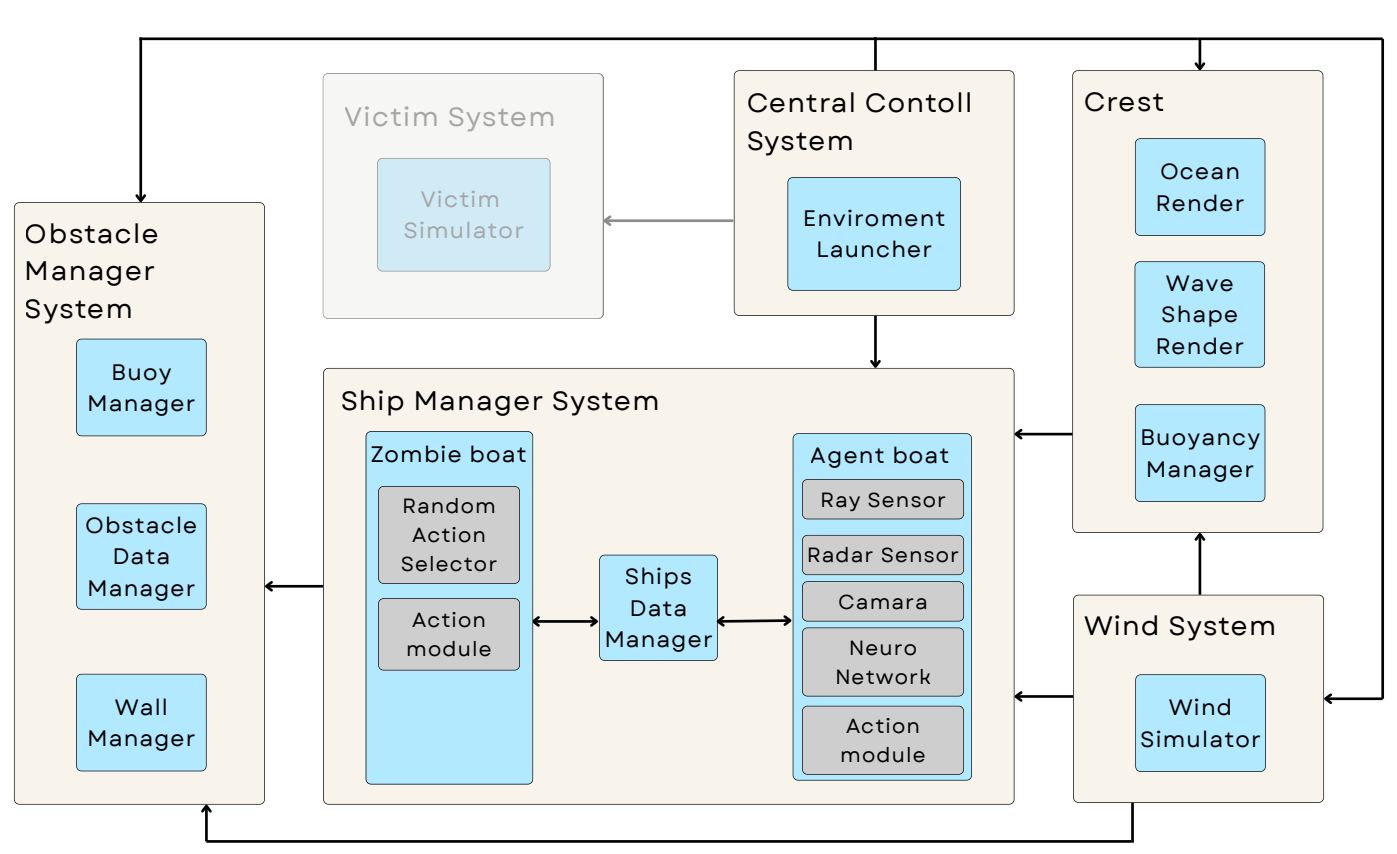
\includegraphics[scale=0.5]{image/TrainingArchitecture.png}
    \caption{訓練環境架構示意圖}
    \label{fig:training_env}
\end{figure}

\newpage

\begin{figure}[h]
    \centering
    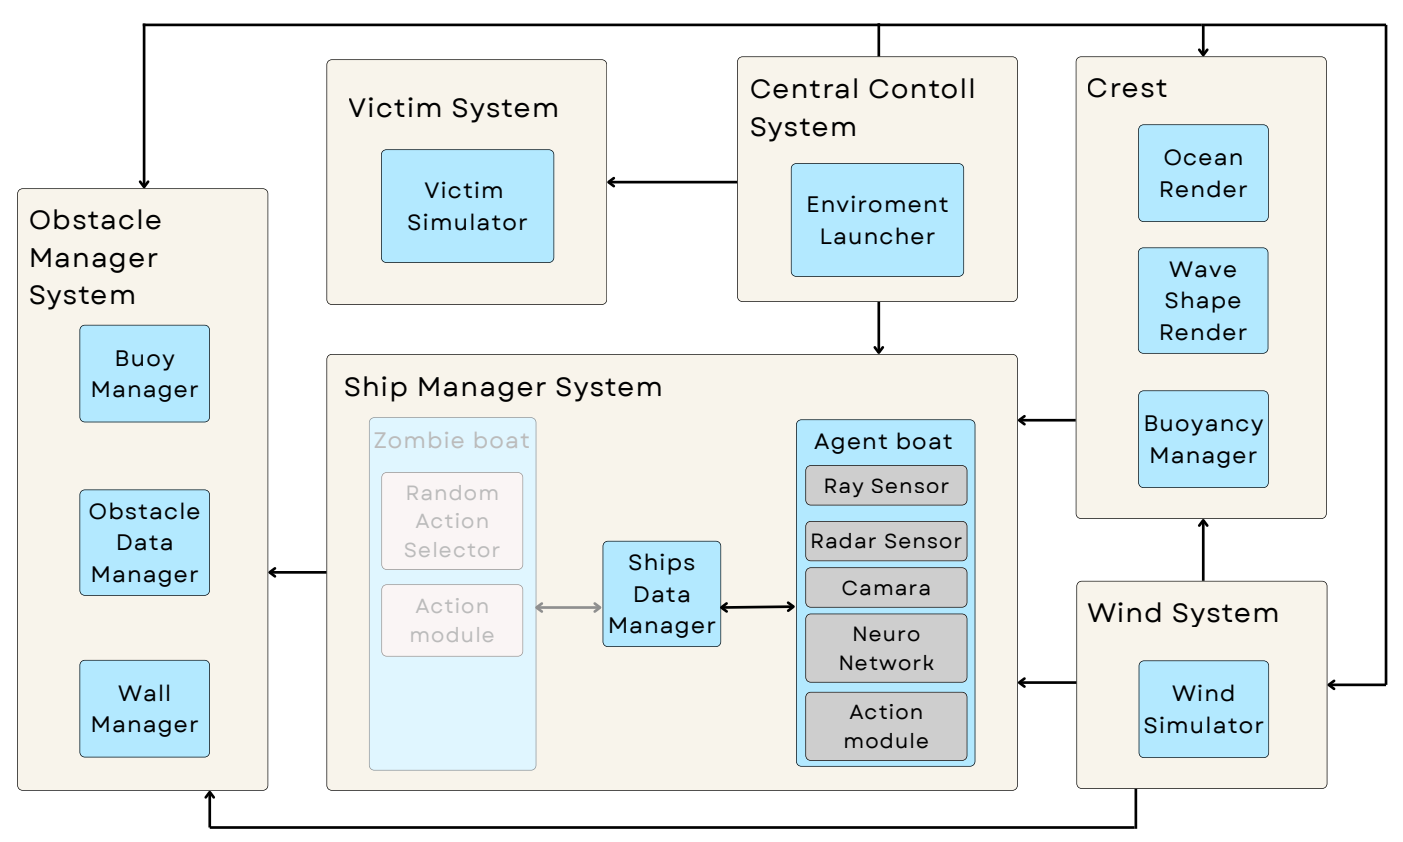
\includegraphics[scale=0.5]{image/SimulationArchitecture.png}
    \caption{模擬救援環境架構示意圖}
    \label{fig:simulation_env}
\end{figure}

\begin{itemize}
	 \item \textbf{中央控制系統 (Central Control System)}
	\begin{itemize}
	    \item \textbf{環境啟動器 (Environment Launcher)}:負責啟動並管理整個環境。
	\end{itemize}
	
	 \item \textbf{船舶管理系統 (Ship Manager System)}
	\begin{itemize}
	    \item \textbf{殭屍船 (Zombie Boat)}:配備隨機動作選擇器與動作模組,作為訓練模式中的虛擬代理。
	    \item \textbf{智能船 (Agent Boat)}:訓練後的智能代理,配備射線感測器、雷達感測器、攝影機、神經網路與動作模組。
	    \item \textbf{船舶資料管理器 (Ships Data Manager)}:統一管理兩種船舶資料,例如當前位置、航向等。
	\end{itemize}
	
	 \item \textbf{波浪系統 (Crest)}
	\begin{itemize}
	    \item \textbf{海洋渲染器 (Ocean Render)}:負責生成整個海洋。
	    \item \textbf{波浪形狀渲染器 (Wave Shape Render)}:產生波浪的元件。
	    \item \textbf{浮力管理器 (Buoyancy Manager)}:處理物體在水中的浮力計算。
	\end{itemize}
	
	 \item \textbf{障礙物管理系統 (Obstacle Manager System)}
	\begin{itemize}
	    \item \textbf{浮標管理器 (Buoy Manager)}:生成及設定障礙物參數,包括是否隨機、跟隨海浪飄移等。
	    \item \textbf{障礙物資料管理器 (Obstacle Data Manager)}:統一管理所有障礙物資料。
	    \item \textbf{牆壁管理器 (Wall Manager)}:生成牆壁障礙物。
	\end{itemize}
	
	 \item \textbf{風力系統 (Wind System)}
	\begin{itemize}
	    \item \textbf{風力模擬器 (Wind Simulator)}:模擬海風,以重現更真實的搜救情境。
	\end{itemize}
	
	 \item \textbf{遇難者系統 (Victim System)}
	\begin{itemize}
	    \item \textbf{遇難者生成模擬器 (Victim Simulator)}:負責生成每次模擬中的遇難者。
	\end{itemize}
	
	 \item \textbf{系統與模組間的相互關係}
	\begin{itemize}
	    \item 船舶管理系統與障礙物管理系統互相溝通,以避免障礙物生成的位置過於靠近船隻。
	    \item 波浪系統影響船舶管理系統中船隻的物理特性。
	    \item 波浪系統影響障礙物管理系統中障礙物的物理特性。
	    \item 風力系統影響多個系統中各個物件的物理特性。
	\end{itemize}

\end{itemize}

\subsection{強化學習架構}
(數學公式我不太想打)

\section{實驗設計與結果分析}

\subsection{實驗環境架設}
本實驗的模擬環境由 Unity 遊戲引擎及 Crest 海洋物理引擎結合而成,得以表現出真實的海面動態與船舶的物理特性。為測試自主船舶在不同情境下的效能,我們在環境中加入了多個變因:
\begin{itemize}
    \item 遇難者的位置:單個、多個或隨機生成
    \item 動態障礙物:漂浮物、其他搜救船隻等
    \item 搜索區域大小與分塊方式
\end{itemize}
透過上述條件組合與調整,我們得以評估自主船舶在海洋環境中的表現與穩定性。

\subsection{模型訓練概述}
\subsubsection{訓練目標}
我們使用 SAC 深度強化學習演算法進行模擬訓練,旨在讓自主船舶具有導航能力與穩定避障的能力。因此在訓練的過程中,我們特別重視船舶的兩種指標:
\begin{itemize}
    \item 任務完成時長:船隻由初始位置到目標點所需時間
    \item 碰撞次數:船隻與障礙物碰撞次數
\end{itemize}
訓練過程中,我們著重於降低兩者的數值,以確保船舶能在多變且複雜的條件下能夠維持良好的表現,並且得以完成任務目標。

\subsubsection{訓練環境的架設}
本實驗的訓練環境以 Unity 與 Crest 海洋物理引擎為基礎,模擬出真實的海面,包括風浪、風速及動態的障礙物,以提供船隻導航及避障所需的複雜環境。我們在場景中配置一個訓練船隻,並加入多艘「zombine boat」作為其他代理人的替代品,這些船隻會隨機行動,模擬多代理系統的互動行為。
值得注意的是,雖然整體系統設計為多代理人系統,但直接訓練多代理人系統會使環境過於複雜,使收斂時間過長,甚至可能無法收斂,而我們的訓練目標僅是船隻的避障與導航,不會涉及代理間的合作。因此我們採用了單代理人的訓練方式,結合上述的 zombie boat 模擬多代理環境,既能節省資源,又能讓代理學習多代理系統下的避障與導航策略。

\subsubsection{訓練流程}
我們的訓練環境以 Unity + Crest 為主,結合 ML-Agents 深度強化學習框架,讓自主船舶能在真實的海面條件下學習避障與導航能力。整個流程可以分為以下階段:
\begin{enumerate}
    \item \textbf{環境初始化}:配置船隻、目標點、障礙物與 \textit{zombie boat}。
    \item \textbf{深度強化學習訓練}:透過 ML-Agents 啟動訓練流程,並採用 SAC 演算法進行訓練,訓練目標為讓船隻從初始位置移動到目標點,同時,在途中不能碰到障礙物或是 zombie boat。
    \item \textbf{訓練監控與紀錄}:使用 TensorBoard 監控訓練過程,包括回合獎勵、碰撞事件與成功到達目的地的次數。
    \item \textbf{模型測試與驗證}:將訓練完成的模型部屬於模擬場景中,測試其在不同環境下的避障與導航表現。
    \item \textbf{結果分析與策略優化}:根據訓練與測試的結果,分析模型在各方面的效能。
\end{enumerate}

\subsection{模擬任務設計與實驗方法}
為了評估自主船舶的表現,我們設計了以下兩種任務類型,以模擬實際情況中自主船舶的實際應用:

\subsubsection{單一落水點快速救援}
這個情景用來模擬單一人員落海的情況,例如郵輪乘客落海、近岸游泳者被離岸流捲走、或是小型漁船翻覆導致單人落水等情景。該情境強調時間的敏感性及位置的不確定性,船隊需要經過仔細的搜尋,在最快的時間內定位落水的人員,並進行施救。
\\ \par
在這個情景下,我們使用以下方法設定我們的環境:
\begin{itemize}
    \item 遇難者定位:位置不明,只知道大概的範圍。
    \item 實驗參數:
    \begin{itemize}
        \item 偵測半徑:
        \item 船隻數量:
        \item time-out:
        \item 海象等級:
        \item 障礙物密集度:
    \end{itemize}
    \item 終止條件與成功判定:
    \begin{itemize}
        \item 成功:任一船隻找到落水者並標記,在 time-out 前完成。
        \item 終止:超過 time-out、發生嚴重碰撞等。
    \end{itemize}
    \item 示意圖
\end{itemize}

\subsubsection{大範圍隨機搜尋任務}
此情景用來模擬在大面積海域中進行隨機分布的搜救任務,例如海上船舶遇難、飛機海面迫降等等。該情境強調搜尋的覆蓋範圍與船體之間的配合,船隊需要再目標數量與位置不明確的情況下,盡可能的提高搜尋效率與範圍覆蓋率,同時也要降低碰撞的風險。
\\ \par
在這個情景下,我們使用以下的方法設定模擬環境:
\begin{itemize}
    \item 目標分布:多個目標隨機生成於整個搜索區域,位置與數量隨機。
    \item 實驗參數:
    \begin{itemize}
        \item 偵測半徑:
        \item 船隻數量:
        \item time-out:
        \item 海象等級:
        \item 障礙物密集度:
    \end{itemize}
    \item 終止條件與成功判定:
    \begin{itemize}
        \item 成功:船隻找到所有落水人員並標記,在 time-out 前完成。
        \item 終止:超過 time-out、發生嚴重碰撞等。
    \end{itemize}
    \item 示意圖
\end{itemize}

\subsubsection{任務效能評估}
有了以上兩種情境後,我們根據我們的需求制定了一系列的評估指標來量化船隊在搜尋任務中的表現。主要指標包括:
\begin{itemize}
    \item 標記時間:指從任務開始到落水者被成功定位的總時間。
    \item 成功救援率:在任務時間的限制內,船隊成功找到落水者的比例。
    \item 碰撞次數:船隻之間或與障礙物發生直接接觸的次數。
    \item 搜尋覆蓋程度:船隊在搜尋任務中實際搜尋的範圍。
    \item 資源使用量:包括船隻的航程長度及估算的資源消耗。
\end{itemize}

以上的指標除了量化船隊在救援上的表現外,也同時得以反映任務中錯誤的發生率。透過對這些指標進行系統化的分析,我們設計了以下的終極目標,以確保在實際應用中既能提高救援效率,又能控制風險與資源消耗:
\begin{itemize}
    \item 最小化標記時間:確保船隊能在最短的時間內完成任務。
    \item 提高成功救援率:增加船隊的可靠性及穩定性。
    \item 降低碰撞次數:提升船隊作業的安全性,減少意外風險。
    \item 提高搜尋覆蓋程度:確保區域被充分搜尋,降低目標遺漏的機率。
    \item 增加救援人數與資源使用量的比值 (待討論):提升資源運用效率。
\end{itemize}

\subsubsection{實驗流程}
\begin{enumerate}
    \item 根據以上兩種情境設定參數:包括船隻數量、偵測半徑、障礙物密度等等,確保模擬場景能夠模擬出多種真實情況。
    \item 部屬船隊於初始位置準備開始:船隻將自行到達初始位置,並等待所有船隻就位,確保所有船隻同時開始搜尋。
    \item 開始進行搜尋,每艘船分別執行合作搜尋任務:船隊依據既定的策略及路徑,開始進行搜尋。
    \item 紀錄相關數據以利未來做分析:(我們輸出了甚麼資料這裡寫一下)
    \item 重複模擬多次,以獲取大量數據進行分析:透過不同的環境重複實驗,確保結果可靠,並進行進一步的分析。
\end{enumerate}

\subsection{實驗結果呈現}
\subsubsection{單一落水點快速救援}
(數據)

\subsubsection{大範圍隨機搜尋任務}
(數據)



\section{結論與未來發展}

\subsection{研究總結}
本專題針對「海上搜救」所面臨的廣域範圍、高不確定性等挑戰,提出並實作一套「智慧化船舶群集搜救系統」。核心成果如下:
\begin{itemize}
    \item \textbf{建立擬真測試平台}:本專案以 Unity 為主要的開發環境,並結合 Crest 海洋模擬套件,模擬真實風浪與海象。這個組合能夠支援大範圍的海洋場景,並兼顧視覺化與即時模擬的效能,非常適合用於實現海上搜救場景的模擬。
    \item \textbf{開發自主搜救船隻}:使用 ML-Agents 與 DQN 演算法訓練出具備自主導航、避障能力的搜救船隻。
    \item \textbf{設計群集協同策略}:針對多艘船舶進行協同搜尋與任務分配,提升搜救效率。
    \item \textbf{驗證可行性}:透過模擬測試驗證系統在不同海象及搜救場景下的可行性。
\end{itemize}

\subsection{專題成果與限制}
% 在此補充系統的成果與目前限制

\subsection{未來研究方向}
% 在此補充後續可進一步探討的方向

\subsection{可行的解決方案}
% 在此補充對目前限制的改善方案或建議

% 參考文獻
\begin{thebibliography}{9}

\bibitem{IAMSAR2008}
IMO,
``IAMSAR Manual Volume II: Mission Co-ordination,''
\textit{International Maritime Organization},
2008.

\bibitem{IAMSAR2016}
IMO,
``IAMSAR Manual Volume III: Mobile Facilities,''
\textit{International Maritime Organization},
2016.

\bibitem{Oways}
Oways,
``IAMSAR Search Patterns,''
\textit{Oways Online},
n.d.
[Online]. Available: \url{https://owaysonline.com/iamsar-search-patterns/}

\bibitem{rybchak2024}
Z.~Rybchak and M.~Kopylets,
``Comparative Analysis of DQN and PPO Algorithms in UAV Obstacle Avoidance 2D Simulation,''
2024.

\bibitem{greenberg}
V.~Greenberg and C.~Hernandez,
``Autonomous Drone Navigation for First Response,''
n.d.

\bibitem{Drew2021}
D.~S.~Drew,
``Multi-Agent Systems for Search and Rescue Applications,''
2021.

\bibitem{LowAltitude2025}
低空经济,
``智能无人机集群协同控制系统设计方案,''
2025年4月27日.
[Online]. Available: \url{https://owaysonline.com/iamsar-search-patterns/}

\bibitem{Fan2023}
范嘉軒,
``虛實整合訓練框架:使用強化學習、Unity3D及ROS2的無人車自動導航,''
2023.

\bibitem{Ericyangyu}
Ericyangyu,
``PPO-for-Beginners,''
GitHub repository,
n.d.
[Online]. Available: \url{https://github.com/ericyangyu/PPO-for-Beginners}


\bibitem{Idrees}
Idreesshaikh,
``Autonomous Driving in Carla Using Deep Reinforcement Learning,''
GitHub repository,
n.d.
[Online]. Available: \url{https://github.com/idreesshaikh/Autonomous-Driving-in-Carla-using-Deep-Reinforcement-Learning?utm\_source=chatgpt.com}


\bibitem{TimeLimits2017}
``Time Limits in Reinforcement Learning,''
2017.

\bibitem{Leurent2019}
Leurent,
``Approximate Planning in POMDPs with Safe Reinforcement Learning,''
2019.

\end{thebibliography}

\end{document}